\documentclass[14pt]{beamer}

\title{Goats and Tiger}
\subtitle{Team 11}

\author[]{BH. Sai Sruthi: 19WH1A0227: EEE \newline P. Pratyusha: 19WH1A0528: CSE \newline K. Sritulasi: 19WH1A0488: ECE \newline S. Sai Harshitha: 19WH1A1253: IT \newline G. Neha: 19WH1A05E4: CSE \newline Chennupati Madhuri: 20WH1A1208: IT}

\date{March 22, 2021}

\usetheme{CambridgeUS}
\usecolortheme{dolphin}
\usepackage{graphicx}
\usepackage{grffile}
\usepackage{hyperref}

\begin{document}
\begin{frame}
	\titlepage
\end{frame}
\begin{frame}{Introduction}
	\begin{itemize}
		\item Bagha Chal or Moving Tiger is an ancient Nepali board game.
		\item It is a strategic 2-player game.
	\end{itemize}
\end{frame}

\begin{frame}{Structure of game board}
	3 Tigers and 15 goats
	\begin{center}
		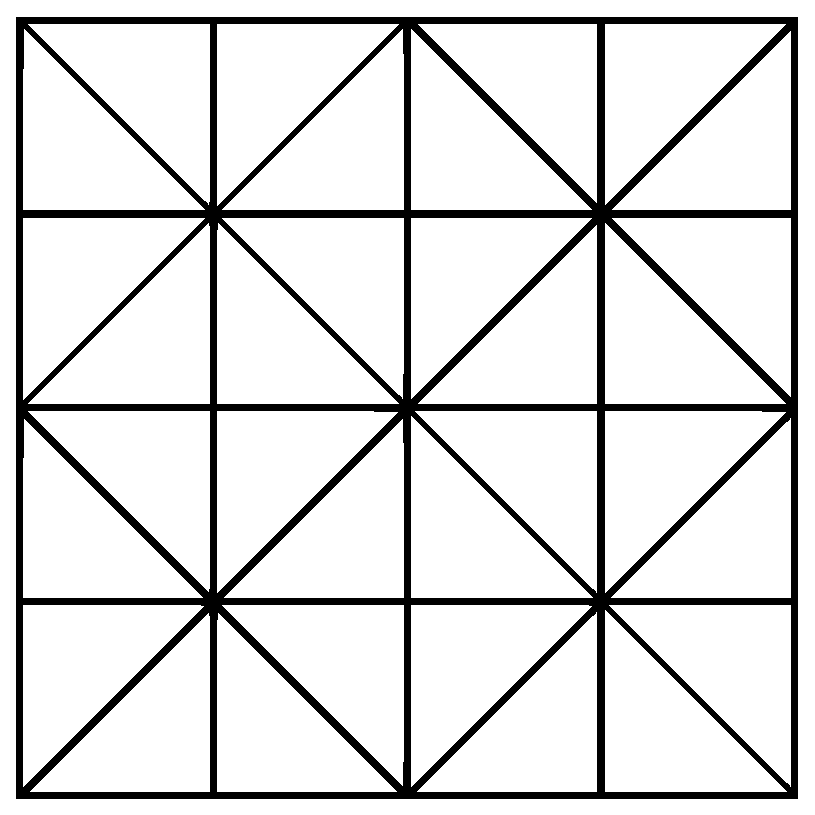
\includegraphics[width=4cm, height=4cm]{goatsTiger_conv.eps}
	\end{center}
\end{frame}
\begin{frame}{Approach}
	\begin{itemize}
		\item Understand the problem statement
		\item Setup the workspace
		\item Decide on the design
		\item Learn Pygame
		\item Collect resources
		\item Start coding
	\end{itemize}
\end{frame}

\begin{frame}{Tech Stack}
	\begin{itemize}
		\item Pygame
        	\item PyCharm
		\item Git
        	\item LaTeX
	\end{itemize}
\end{frame}

\begin{frame}{Learnings}
	\begin{itemize}
		\item LaTeX
		\item Team collaboration
		\item Game play
	\end{itemize}
\end{frame}

\begin{frame}{Challenges}
	\begin{itemize}
		\item Setting up PyGame
		\item Compiling tex files
	\end{itemize}
\end{frame}

\begin{frame}
	\begin{center}
	\textbf{\huge Thank You!}
	\end{center}
\end{frame}

\end{document}
	

